\documentclass[11pt]{article}

% Language setting
\usepackage[spanish, es-noquoting, es-noshorthands]{babel}
\usepackage[T1]{fontenc}
\usepackage[utf8]{inputenc}
\usepackage{lmodern}
\usepackage{microtype}

% Set page size and margins
\usepackage[letterpaper,top=2cm,bottom=2cm,left=3cm,right=3cm,marginparwidth=1.75cm]{geometry}

% Useful packages
\usepackage{amsmath, amssymb, amsthm, mathtools}
\usepackage{graphicx}
\usepackage[colorlinks=true, allcolors=blue]{hyperref}
\usepackage[capitalise]{cleveref}
\usepackage{enumitem}
\usepackage{multicol}

% Macros for common mathematical symbols
\newcommand{\N}{\mathbb{N}}
\newcommand{\Z}{\mathbb{Z}}
\newcommand{\Q}{\mathbb{Q}}
\newcommand{\R}{\mathbb{R}}
\newcommand{\C}{\mathbb{C}}

\title{\textbf{Guía Álgebra - Práctica 1}}
\author{Lorenzo Durante}
\date{}

\begin{document}
\maketitle

\section{Introducción}
Esta es la resolución de la primera guía de ejercicios de Álgebra 1 para Ciencias de la Computación en la UBA.

\section{Conjuntos}
\subsection{Dado el conjunto \(A = \{ 1, 2, 3\}\), determinar cuáles de las siguientes afirmaciones son verdaderas.}

\begin{enumerate}[label=\roman*)]
    \item \(1 \in A\)
    \item \(\{1\} \subseteq A\)
    \item \(\{2,1\} \subseteq A\)
    \item \(\{1,3\} \in A\)
    \item \(\{2\} \in A\)
\end{enumerate}

\textbf{Resolución}

\begin{enumerate}[label=\roman*)]
    \item \(1 \in A\): el número \(1\) pertenece al conjunto \(A\). \textbf{(Verdadero)}
    \item \(\{1\} \subseteq A\): todos los elementos de \(\{1\}\) pertenecen a \(A\). \textbf{(Verdadero)}
    \item \(\{2,1\} \subseteq A\): \(1\) y \(2\) pertenecen a \(A\). \textbf{(Verdadero)}
    \item \(\{1,3\} \notin A\): \(A\) no contiene al conjunto \(\{1,3\}\) como \emph{elemento}. \textbf{(Verdadero)}
    \item \(\{2\} \notin A\): el elemento \(\{2\}\) no pertenece a \(A\). \textbf{(Verdadero)}
\end{enumerate}

\subsection{Dado el conjunto \(A = \{1, 2, \{3\}, \{1,2\}\}\), determinar cuáles de las siguientes afirmaciones son verdaderas.}

\begin{multicols}{2}
\begin{enumerate}[label=\roman*)]
    \item \(3 \in A\)
    \item \(\{3\} \subseteq A\)
    \item \(\{3\} \in A\)
    \item \(\{\{3\}\} \subseteq A\)
    \item \(\{1,2\} \in A\)
    \item \(\{1,2\} \subseteq A\)
    \item \(\{\{1,2\}\} \subseteq A\)
    \item \(\{\{1,2\}, 3\} \subseteq A\)
    \item \(\emptyset \in A\)
    \item \(\emptyset \subseteq A\)
    \item \(A \in A\)
    \item \(A \subseteq A\)
\end{enumerate}
\end{multicols}

\textbf{Resolución}
\begin{enumerate}[label=\roman*)]
    \item \(3 \notin A\). \textbf{Falso} que \(3 \in A\).
    \item \(\{3\} \not\subseteq A\). \textbf{Falso} que \(\{3\}\subseteq A\).
    \item \(\{3\} \in A\). \textbf{Verdadero}.
    \item \(\{\{3\}\} \subseteq A\). \textbf{Verdadero}.
    \item \(\{1,2\} \in A\). \textbf{Verdadero}.
    \item \(\{1,2\} \subseteq A\). \textbf{Verdadero}.
    \item \(\{\{1,2\}\} \subseteq A\). \textbf{Verdadero}.
    \item \(\{\{1,2\},3\} \not\subseteq A\) porque \(3\notin A\). \textbf{Falso} que sea subconjunto.
    \item \(\emptyset \in A\). \textbf{Falso}.
    \item \(\emptyset \subseteq A\). \textbf{Verdadero}.
    \item \(A \in A\). \textbf{Falso}.
    \item \(A \subseteq A\). \textbf{Verdadero}.
\end{enumerate}

\subsection{Determinar si \(A \subseteq B\) en cada uno de los siguientes casos.}

\begin{enumerate}[label=\roman*)]
    \item \(A = \{1,2,3\}, \quad B = \{5,4,3,2,1\}\)
    \item \(A = \{1,2,3\}, \quad B = \{1,2,\{3\},-3\}\)
    \item \(A = \{x \in \R \mid 2 < |x| < 3\}, \quad B = \{x \in \R \mid x^2 < 3\}\)
    \item \(A = \{\emptyset\}, \quad B = \emptyset\)
\end{enumerate}

\textbf{Resolución}
\begin{enumerate}[label=\roman*)]
    \item \(A \subseteq B\).
    \item \(A \not\subseteq B\) (porque \(3\notin B\)).
    \item \(A \not\subseteq B\). En efecto,
    \[
      A = (-3,-2)\,\cup\,(2,3),\qquad
      B = (-\sqrt{3}, \sqrt{3}),
    \]
    y, por ejemplo, \(-2{,}5 \in A\) pero \(-2{,}5 \notin B\).
    \item \(A \not\subseteq B\) (porque \(\emptyset\notin \emptyset\)).
\end{enumerate}

\subsection{Dados los subconjuntos}
\begin{align*}
A &= \{1,-2,7,3\}, \\
B &= \{1,\{3\},10\}, \\
C &= \{-2,\{1,2,3\},3\}
\end{align*}
del conjunto referencial
\[
V = \{1,\{3\},-2,7,10,\{1,2,3\},3\},
\]
hallar
\begin{enumerate}[label=\roman*)]
  \item \(A \cap (B \triangle C)\)
  \item \((A \cap B)\triangle (A \cap C)\)
  \item \(A^{c}\cap B^{c}\cap C^{c}\)
\end{enumerate}

\textbf{Resolución}
\begin{enumerate}[label=\roman*)]
    \item \(A \cap (B \triangle C) = \{1, -2, 3\}\).

    \item \((A \cap B) \triangle (A \cap C) = \{1, -2, 3\}\).
    \[
      A\cap B=\{1\},\qquad A\cap C=\{-2,3\}.
    \]

    \item \(A^{c} \cap B^{c} \cap C^{c} = \emptyset\). Con \(V\) como referencial:
    \[
      A^{c}=\{\{3\},10,\{1,2,3\}\},\;
      B^{c}=\{-2,7,\{1,2,3\},3\},\;
      C^{c}=\{1,\{3\},7,10\}.
    \]
    La intersección es vacía.
\end{enumerate}

\subsection{Dados subconjuntos \(A, B, C\) de un conjunto referencial \(V\), describir 
\((A \cup B \cup C)^{c}\) en términos de intersecciones y complementos, 
y \((A \cap B \cap C)^{c}\) en términos de uniones y complementos.}

\textbf{Resolución.} (Leyes de De Morgan)
\[
    (A \cup B \cup C)^{c} = A^{c} \cap B^{c} \cap C^{c},
    \qquad
    (A \cap B \cap C)^{c} = A^{c} \cup B^{c} \cup C^{c}.
\]

\subsection{Sean \(A\), \(B\) y \(C\) conjuntos. Representar en un diagrama de Venn}

\begin{multicols}{3}
\begin{enumerate}[label=\roman*)]
    \item \((A \cup B^{c}) \cap C\)
    \item \(A \triangle (B \cup C)\)
    \item \(A \cup (B \triangle C)\)
\end{enumerate}
\end{multicols}

Completado en hoja.

\subsection{Encontrar fórmulas que describan las partes rayadas de los siguientes diagramas de Venn, utilizando únicamente intersecciones, uniones y complementos.}
\begin{figure}[h!]
    \centering
    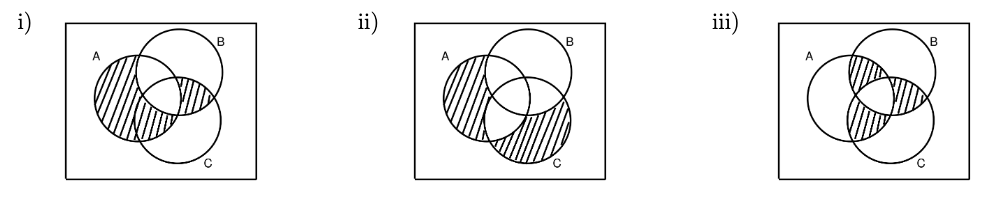
\includegraphics[width=1\textwidth]{image.png}
    \caption{Diagramas de Venn}
    \label{fig:venn}
\end{figure}

\textbf{Resolución}
\begin{enumerate}[label=\roman*)]
    \item \((B^{c} \cap A) \cup (A^{c} \cap C \cap B)\)
    \item \textit{(Revisar con el diagrama)} \((A \cap B^{c} \cap C^{c}) \cup (A^{c} \cap B^{c} \cap C)\)
    \item \((C^{c} \cap B \cap A) \cup (A^{c} \cap B \cap C) \cup (B^{c} \cap A \cap C)\)
\end{enumerate}

\subsection{Hallar el conjunto \(P(A)\) de partes de \(A\) en los casos}
\begin{multicols}{3}
    \begin{enumerate}[label=\roman*)]
        \item \(A = \{1\}\)
        \item \( A = \{a, b\}\)
        \item \(A = \{1, \{1, 2\}, 3\}\)
    \end{enumerate}
\end{multicols}

\textbf{Resolución}

\begin{enumerate}[label=\roman*)]
    \item \(P(A) = \{\emptyset, \{1\}\}\)
    \item \(P(A) = \{\emptyset, \{a\}, \{b\}, \{a, b\}\}\)
    \item \(P(A) = \{\emptyset, \{1\}, \{\{1,2\}\}, \{3\}, \{1, \{1,2\}\}, \{1, 3\}, \{\{1,2\}, 3\}, \{1, \{1,2\}, 3\}\}\)
\end{enumerate}

\subsection{Sean \(A\) y \(B\) conjuntos. Probar que \(P(A) \subseteq P(B) \Leftrightarrow A \subseteq B\).}

\textbf{Demostración.}
\emph{(\(\Rightarrow\))} Si \(P(A)\subseteq P(B)\) entonces, como \(A\in P(A)\), se tiene \(A\in P(B)\), luego \(A\subseteq B\).
\emph{(\(\Leftarrow\))} Si \(A\subseteq B\) y \(X\in P(A)\), entonces \(X\subseteq A\subseteq B\), por lo tanto \(X\in P(B)\). Concluye \(P(A)\subseteq P(B)\).

\subsection{Sean \(p, q\) proposiciones. Verificar que las siguientes expresiones tienen la misma tabla de verdad para concluir que son equivalentes.}

\begin{enumerate}[label=\roman*)]
\item \(p \Rightarrow q\), \quad \(\neg q \Rightarrow \neg p\), \quad \(\neg p \lor q\) \quad y \quad \(\neg (p \land \neg q)\).

Esto permite demostrar \(p \Rightarrow q\) probando en su lugar 
\(\neg q \Rightarrow \neg p\) (contrarrecíproco), 
o probando \(\neg (p \land \neg q)\) (reducción al absurdo).

\item \(\neg (p \Rightarrow q)\) \quad y \quad \(p \land \neg q\).
\end{enumerate}

\textbf{Resolución}
\begin{enumerate}[label=\roman*)]
   \item
\[
\begin{array}{|c|c|c|}
\hline
p & q & p \rightarrow q \\
\hline
V & V & V \\
V & F & F \\
F & V & V \\
F & F & V \\
\hline
\end{array}
\qquad
\begin{array}{|c|c|c|}
\hline
p & q & \neg q \rightarrow \neg p \\
\hline
V & V & V \\
V & F & F \\
F & V & V \\
F & F & V \\
\hline
\end{array}
\]
\[
\begin{array}{|c|c|c|}
\hline
p & q & \neg p \lor q \\
\hline
V & V & V \\
V & F & F \\
F & V & V \\
F & F & V \\
\hline
\end{array}
\qquad
\begin{array}{|c|c|c|}
\hline
p & q & \neg (p \land \neg q) \\
\hline
V & V & V \\
V & F & F \\
F & V & V \\
F & F & V \\
\hline
\end{array}
\]
Todas coinciden, por lo tanto son equivalentes.

\item 
\[
\begin{array}{|c|c|c|}
    \hline
    p & q & \neg(p \rightarrow q) \\
    \hline
    V & V & F \\
    V & F & V \\
    F & V & F \\
    F & F & F \\
    \hline
\end{array}
\qquad
\begin{array}{|c|c|c|}
    \hline
    p & q & p \land \neg q \\
    \hline
    V & V & F \\
    V & F & V \\
    F & V & F \\
    F & F & F \\
    \hline
\end{array}
\]
Es equivalente.
\end{enumerate}

\subsection{Hallar contraejemplos para mostrar que las siguientes proposiciones son falsas.}

\begin{enumerate}[label=\roman*)]
    \item \(\forall a \in \N,\; \dfrac{a-1}{a}\) no es un número entero.
    \item \(\forall x, y \in \R\) con \(x,y>0,\; \sqrt{x+y} = \sqrt{x} + \sqrt{y}\).
    \item \(\forall x \in \R,\; x^2 > 4 \Rightarrow x > 2\).
\end{enumerate}

\textbf{Resolución}
\begin{enumerate}[label=\roman*)]
    \item Tomando \(a=1\): \(\dfrac{1-1}{1}=0\in\Z\). (Contraejemplo)
    \item Tomando \(x=y=1\): \(\sqrt{2}\neq 1+1\). (Contraejemplo)
    \item Tomando \(x=-3\): \(x^2=9>4\) pero \(-3\not>2\). (Contraejemplo)
\end{enumerate}

\subsection{}

\begin{enumerate}[label=\roman*)]
    \item Decidir si las siguientes proposiciones son verdaderas o falsas, justificando debidamente.
    \begin{enumerate}[label=(\alph*)]
        \item $\forall n \in \mathbb{N}, \; n \geq 5 \; \lor \; n \leq 8.$
        \item $\exists n \in \mathbb{N} \; / \; n \geq 5 \; \land \; n \leq 8.$
        \item $\forall n \in \mathbb{N}, \; \exists m \in \mathbb{N} \; / \; m > n.$
        \item $\exists n \in \mathbb{N} \; / \; \forall m \in \mathbb{N}, \; m > n.$
        \item $\forall x \in \mathbb{R}, \; x > 3 \; \Rightarrow \; x^2 > 4.$
        \item Si $n$ es un número natural terminado en $4$, entonces $n$ es par.
    \end{enumerate}

    \item Negar las proposiciones anteriores, y en cada caso verificar que la proposición negada tiene el valor de verdad opuesto al de la original.

    \item Reescribir las proposiciones \textbf{e)} y \textbf{f)} del ítem i) utilizando las equivalencias del ejercicio 10i).
\end{enumerate}

\begin{enumerate}[label=\roman*)]
    \item \begin{enumerate}
        \item Esta proposición es \textbf{verdadera}, ya que para todo $n \in \mathbb{N}$ siempre se cumple al menos una de las condiciones. 
        Si $n < 5$, entonces $n \leq 8$ es cierto; y si $n \geq 5$, se cumple la primera condición. 
        No existe valor de $n$ que invalide ambas.
        
        \item La proposición es \textbf{verdadera} porque todos los números naturales  cumplen simultáneamente $n \geq 5$ y $n \leq 8$. 
        Por ejemplo, $n=6$ satisface ambas condiciones, por lo que la proposición es cierta.

        \item La proposición es \textbf{falsa} porque siempre se puede elegir $m = n$ lo que contradice la proposición.

        \item La proposición es \textbf{falsa} por el mismo motivo del item anterior. Siempre se puede elegir $m = n$.

        \item La proposición es \textbf{falsa} porque si $x = 1$, $1 > 3$ es falsO y $1^{2} > 4$ es nuevamente falso por lo que la proposición es falsa.

        \item La proposición es \textbf{falsa}.
    \end{enumerate}

\begin{enumerate}
  \item
  \begin{enumerate}
    \item 
    \begin{align*}
      \neg \big(\forall n \in \mathbb{N}\;\mid\; n \ge 5 \,\lor\, n \le 8\big) \\
      \equiv\ \exists n \in \mathbb{N}\;\mid\; \neg(n \ge 5 \,\lor\, n \le 8) \\
      \equiv\ \exists n \in \mathbb{N}\;\mid\; (n < 5) \,\land\, (n > 8)
    \end{align*}
  \end{enumerate}
  La negación es imposible, no existe un posible valor de $n$ que sea a la misma vez menos que 5 y mayor que 8. Que sea imposible, confirma que la proposición original es \textbf{verdadera}.
  \item
    \begin{align*}
        \forall n \in \mathbb{N} \;\mid\; \neg(n \geq 5 \lor n \leq 8) \\
        \equiv \forall n \in \mathbb{N} \;\mid\; (n < 5 \land n > 8)
    \end{align*}
    La negación es imposible por lo que se confirma que la proposición original es \textbf{verdadera}.
  \item \begin{align*}
    \exists n \in \mathbb{N}, \forall m \in \mathbb{N} \mid \neg (m > n) \\ 
    \equiv \exists n \in \mathbb{N}, \forall m \in \mathbb{N} \mid m \leq n
  \end{align*}
  Esto es verdadero ya que 1 cumple la condición. Esto hace que la negación sea verdadera y confirma que la proposición original es \textbf{falsa}.
  \item \begin{align*}
    \forall n \in \mathbb{N} \mid \exists m \in \mathbb{N}, \neg(m > n )\\
    \forall n \in \mathbb{N} \mid \exists m \in \mathbb{N}, m \leq n
  \end{align*}
  Esta negación es falsa ya que se puede elegir los valores para $n = 1$ y $m = 1$ para que no se cumpla la negación. Esto hace que la proposición original se confirme como \textbf{verdadera}. 
  \item \begin{align*}
    \exists x \in \mathbb{R}, \neg (x > 3 \rightarrow x^{2} > 4)\\
    \exists x \in \mathbb{R}, (x > 3) \land (x^{2} \leq 4)
  \end{align*}
  Esta negación es imposible lo que hace la preposición original \textbf{verdadera}.
  \item Existe un número natural que termina en 4 y no es par. \\
  Esta negación es falsa por lo que la proposición original es \textbf{verdadera}. 
\end{enumerate}
\end{enumerate}
\subsection{Determinar cuáles de las siguientes afirmaciones son verdaderas 
cualesquiera sean los subconjuntos $A$, $B$ y $C$ de un conjunto referencial $V$ 
y cuáles no. Para las que sean verdaderas, dar una demostración, para las otras dar un contraejemplo. }

\begin{enumerate}[label=\roman*)]
  \item $(A \triangle B) - C = (A - C) \triangle (B - C).$
  \item $(A \cap B) \triangle C = (A \triangle C) \cap (B \triangle C).$
  \item $C \subseteq A \;\;\Rightarrow\;\; B \cap C \subseteq (A \triangle B)^c.$
  \item $A \triangle B = \emptyset \;\;\Leftrightarrow\;\; A = B.$
\end{enumerate}

\begin{enumerate}[label=\roman*)]
\item Demostrar que
\[
(A \triangle B) - C \;=\; (A - C) \triangle (B - C).
\]

\textbf{Demostración.} 

\begin{align*}
    (A \triangle B) - C &= (A - C) \triangle (B - C ) \\
    [(A - B) \cup (B - A)] - C &= [(A - C) - (B - C)] \cup [(B - C) - (A - C)] \\
    [(A - B) - C \cup (B - A) - C] &= [A - (B \cup C)] \cup [B - (C \cup A)] \\
    A - (B \cup C) \cup B - (A \cup C) &= A - (B \cup C) \cup B - (A \cup C)
\end{align*}

Las dos expresiones son iguales.

\[
    A = \{1\}, \quad B = \{2\}, \quad C = \{1,3\}.
\]

\item 
\textbf{(i) Lado izquierdo}
\begin{align*}
(A \cap B) \triangle C 
&= \{1\}\cap\{2\} \;\triangle\; \{1,3\} \\
&= \varnothing \;\triangle\; \{1,3\} \\
&= \{1,3\}.
\end{align*}

\textbf{(ii) Lado derecho}
\begin{align*}
(A \triangle C)\cap(B \triangle C) 
&= \big(\{1\}\triangle\{1,3\}\big) \;\cap\; \big(\{2\}\triangle\{1,3\}\big) \\
&= \{3\}\cap\{1,2,3\} \\
&= \{3\}.
\end{align*}

\textbf{Conclusión.} \\
El lado izquierdo resulta en $\{1,3\}$, mientras que el lado derecho resulta en $\{3\}$. 
Por lo tanto, la igualdad no se cumple en este caso, lo que confirma que la proposición no es verdadera en general.

\item Demostrar que 
\[
    C \subseteq A \Rightarrow B \cap C \subseteq (A \triangle B)^{C}
\]
TODO -- FINALIZAR ESTE PUNTO
\end{enumerate}

\subsection{}

Sean $A, B$ y $C$ subconjuntos de un conjunto referencial $V$. Probar que

\begin{enumerate}
    \item $A \cap (B \triangle C) = (A \cap B) \triangle (A \cap C)$.
    \item $A - (B - C) = (A - B) \cup (A \cap C)$.
    \item $A \triangle B \subseteq (A \triangle C) \cup (B \triangle C)$.
    \item $(A \cap B)^{c} \cup (C \cap D)^{c} = (A \cap C)^{c} \cup (B \cap D)^{c}$.
    \item $A \subseteq B \;\Rightarrow\; A \triangle B = B \cap A^{c}$.
    \item $A \cap C = \varnothing \;\Rightarrow\; A \cap (B \triangle C) = A \cap B$.
\end{enumerate}

\begin{enumerate}
    \item \begin{align*}
        A \cup ( B \triangle C) = (A \cap B) \triangle (A \cap C)
    \end{align*}
\end{enumerate}
\subsection{}
\subsection{}

\textbf{Relaciones}
\subsection{Sean $A = \{1,2,3\}$ y $B = \{1,3,5,7\}$. Verificar si las siguientes son relaciones de $A$ en $B$ y en caso afirmativo graficarlas por medio de un diagrama con flechas de $A$ en $B$, y por medio de puntos en el producto cartesiano $A \times B$.}

\begin{enumerate}[label=\roman*)]
    \item $\mathcal{R} = \{(1,1), (1,3), (1,7), (3,1), (3,5)\}$.
    \item $\mathcal{R} = \{(1,1), (1,3), (2,7), (3,2), (3,5)\}$.
    \item $\mathcal{R} = \{(1,1), (2,7), (3,7)\}$.
    \item $\mathcal{R} = \{(1,3), (2,1), (3,7)\}$.
\end{enumerate}
\textbf{Resolución}
\begin{enumerate}[label=\roman*)]
    \item Verdadero. 
    \item Falso.
    \item Verdadero.
    \item Verdadero
\end{enumerate}

\subsection{Sean $A = \{1,2,3\}$ y $B = \{1,3,5,7\}$. Describir por extensión cada una de las relaciones siguientes de $A$ en $B$.}

\begin{enumerate}[label=\roman*)]
    \item $(a,b) \in \mathcal{R} \iff a \leq b$
    \item $(a,b) \in \mathcal{R} \iff a > b$
    \item $(a,b) \in \mathcal{R} \iff a \cdot b \text{ es par}$
    \item $(a,b) \in \mathcal{R} \iff a + b > 6$
\end{enumerate}

\textbf{Resolución}
\begin{enumerate}[label=\roman*)]
    \item $ R_{1} =  \{(1,1), (1, 3), (1, 5), (1, 7), (2, 3), (2, 5), (2, 7), (3, 3), (3, 5), (3, 7)\}$
    \item $ R_{2} = \{ (2,1 ), (3,1)\}$
    \item $ R_{3} = \{(2,1), (2,3) (2, 5), (2, 7)\}$
    \item $ R_{4} = \{(1, 7), (2,5), (2, 7), (3,5), (3,7)\} $
\end{enumerate}

\subsection{Sea $A = \{a, b, c, d, e, f\}$ y sea $\mathcal{R}$ la relación en $A$ representada por el gráfico:}

\begin{center}
    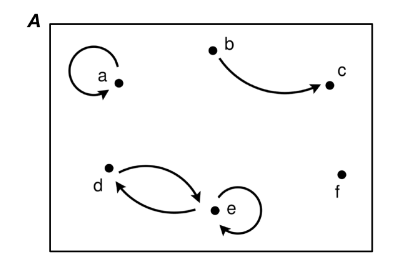
\includegraphics[scale=1]{ejercicio21.png}
\end{center}

Hallar la mínima cantidad de pares que se deben agregar a $\mathcal{R}$ de manera que la nueva relación obtenida sea

\begin{enumerate}[label=\roman*)]
    \item reflexiva,
    \item simétrica,
    \item transitiva,
    \item reflexiva y simétrica,
    \item simétrica y transitiva,
    \item de equivalencia.
\end{enumerate}

\textbf{Resolución}

\begin{enumerate}[label=\roman*)]
    \item 4
    \item 1
    \item 2
    \item 5
    \item 4
    \item 5
\end{enumerate}

\subsection{En cada uno de los siguientes casos determinar si la relación $\mathcal{R}$ en $A$ es reflexiva, simétrica, antisimétrica, transitiva, de equivalencia o de orden.}

\begin{enumerate}[label=\roman*)]
    \item $A = \{1,2,3,4,5\}, \;
    \mathcal{R} = \{(1,1),(2,2),(3,3),(4,4),(5,5),(1,2),(1,3),(2,5),(1,5)\}$.

    \item $A = \mathbb{N}, \;
    \mathcal{R} = \{(a,b)\in \mathbb{N}\times\mathbb{N} \mid a+b \text{ es par}\}$.

    \item $A = \mathbb{Z}, \;
    \mathcal{R} = \{(a,b)\in \mathbb{Z}\times\mathbb{Z} \mid |a|\leq |b|\}$.

    \item $A = \mathbb{Z}, \;
    \mathcal{R}$ definida por $a \,\mathcal{R}\, b \;\Leftrightarrow\; b \text{ es múltiplo de } a$.

    \item $A = \mathcal{P}(\mathbb{R}), \;
    \mathcal{R}$ definida por $X \,\mathcal{R}\, Y \;\Leftrightarrow\; X\cap\{1,2,3\} \subseteq Y\cap\{1,2,3\}$.

    \item $A = \mathcal{P}(\{n\in\mathbb{N}\mid n\leq 30\}), \;
    \mathcal{R}$ definida por $X \,\mathcal{R}\, Y \;\Leftrightarrow\; 2\notin X \cap Y^c$.

    \item $A = \mathbb{N}\times\mathbb{N}, \;\\
    \mathcal{R}$ definida por $(a,b)\,\mathcal{R}\,(c,d) \;\Leftrightarrow\; bc \text{ es múltiplo de } ad$.
\end{enumerate}

\textbf{Resolución}

\begin{enumerate}[label=\roman*)]
    \item Es reflexiva, porque $(x,x)$ para todo $x \in A$, y transitiva porque, por ejemplo, si $(1,2)$ y $(2,5)$ pertenecen a $R$, entonces también $(1,5) \in R$. El "camino" de transitividad se cumple. 

    \item La relación se define como:
    \[
        (a,b) \in R \;\;\Longleftrightarrow\;\; a+b \text{ es par}.
    \]

    Para la reflexividad, reemplazamos $b$ por $a$:
    \[
        a+b \;\longrightarrow\; a+a = 2a,
    \]
    y como $2a$ siempre es par, $(a,a) \in R$ para todo $a \in A$.

    Para la simetría:
    \[
        a+b = b+a,
    \]
    entonces si $(a,b) \in R$, también $(b,a) \in R$.

    También es transitiva (se cumple la condición explicada antes).  

    Por lo tanto, al ser reflexiva, simétrica y transitiva, se concluye que $R$ es una relación de equivalencia.

    \item Es reflexiva, no es simetrica ni antisimetrica y es transitiva.
    \item Es reflexiva, no es simetrica y transitiva
\end{enumerate}
\subsection{Sea $A$ un conjunto. Describir todas las relaciones en $A$ que son a la vez}

\begin{enumerate}[label=\roman*)]
    \item simétricas y antisimétricas.
    \item de equivalencia y de orden.
\end{enumerate}

\begin{enumerate}[label=\roman*)]
    \item Necesita ser: conjunto vacio, relacion con un solo par por ej. $\{(1, 1)\}$ o relacion identidad por ej: \{(1,1), (2,2)\}
    \item $R = \{(a,a): a \in A\}$
\end{enumerate}

\subsection{Sea $A = \{a, b, c, d, e, f\}$. Dada la relación de equivalencia en $A$}

\[
R = \{(a,a),(b,b),(c,c),(d,d),(e,e),(f,f),(a,b),(b,a),(a,f),(f,a),(b,f),(f,b),(c,e),(e,c)\}
\]

hallar la clase $\overline{a}$ de $a$, la clase $\overline{b}$ de $b$, la clase $\overline{c}$ de $c$, 
la clase $\overline{d}$ de $d$, y la partición asociada a $R$.

\begin{enumerate}[]
    \item $\overline{a}$ = $\{a, b, f\}$
    \item $\overline{b}$ = $\{a, b, f, \}$
    \item $\overline{c}$ = $\{c, e \}$
    \item $\overline{d}$ = $\{d\}$
    \item Partición de A: $\{\{a,b,f\},\ \{c,e\},\ \{d\}\}$
\end{enumerate}

\subsection{Sea $A = \{1,2,3,4,5,6,7,8,9,10\}$. Hallar y graficar la relación de equivalencia en $A$ asociada a la partición }
\[
\{\{1,3\},\ \{2,6,7\},\ \{4,8,9,10\},\ \{5\}\}.
\]

¿Cuántas clases de equivalencia distintas tiene? Hallar un representante para cada clase.

\textbf{Resolución} \\
La partición dada es:
\[
\{\{1,3\},\ \{2,6,7\},\ \{4,8,9,10\},\ \{5\}\}.
\]

Por lo tanto, las clases de equivalencia son:
\[
\overline{1} = \{1,3\}, \quad
\overline{2} = \{2,6,7\}, \quad
\overline{4} = \{4,8,9,10\}, \quad
\overline{5} = \{5\}.
\]

\[
\text{Número de clases distintas: } 4.
\]

Un representante de cada clase puede ser, por ejemplo:
\[
1 \in \{1,3\}, \quad
2 \in \{2,6,7\}, \quad
4 \in \{4,8,9,10\}, \quad
5 \in \{5\}.
\]

\subsection{Sean $P=\mathcal{P}(\{1,2,3,4,5,6,7,8,9,10\})$ el conjunto de partes de $\{1,\ldots,10\}$ y $R$ la relación en $P$ definida por}
\[
A \,R\, B \;\Longleftrightarrow\; (A \triangle B)\cap \{1,2,3\}=\varnothing.
\]

\begin{enumerate}[label=\roman*)]
\item Probar que $R$ es una relación de equivalencia y decidir si es antisimétrica. \textit{(Sugerencia: usar adecuadamente el ejercicio 14(iii)).}
\item Hallar la clase de equivalencia de $A=\{1,2,3\}$.
\end{enumerate}

\textbf{Resolución}

\begin{enumerate}[label=\roman*)]
    \item Vamos a escribirlo en palabras. \\
    A es relacion con B si y solo si no existe interseccion entre \{1, 2, 3\} y $A \triangle B$ \\
    Evaluemos la reflexividad
    \begin{align*}
        A R A \Leftrightarrow (A \triangle A) \cap \{1,2,3\} = \emptyset \\
        A R A \Leftrightarrow (\emptyset) \cap \{1,2,3\} = \emptyset \\
        \emptyset = \emptyset 
    \end{align*}
    Esta relación es reflexiva. \\
    La relación es simetrica porque $A \triangle B$ siempre va a ser lo mismo que $ B \triangle A$ \\
    Tambien es transitiva por lo que ahce esta relación \textbf{una relacion de equivalencia}.
    \item Clase de equivalencia = $2^{8}$ combinaciones de $\{1,2,3\}$
\end{enumerate}


\end{document}
